\chapter{Data analysis examples}~\label{appendix-data-analysis-examples}

\epigraph{A sample of the manifold}{anon}

\begin{figure}
    \centering
    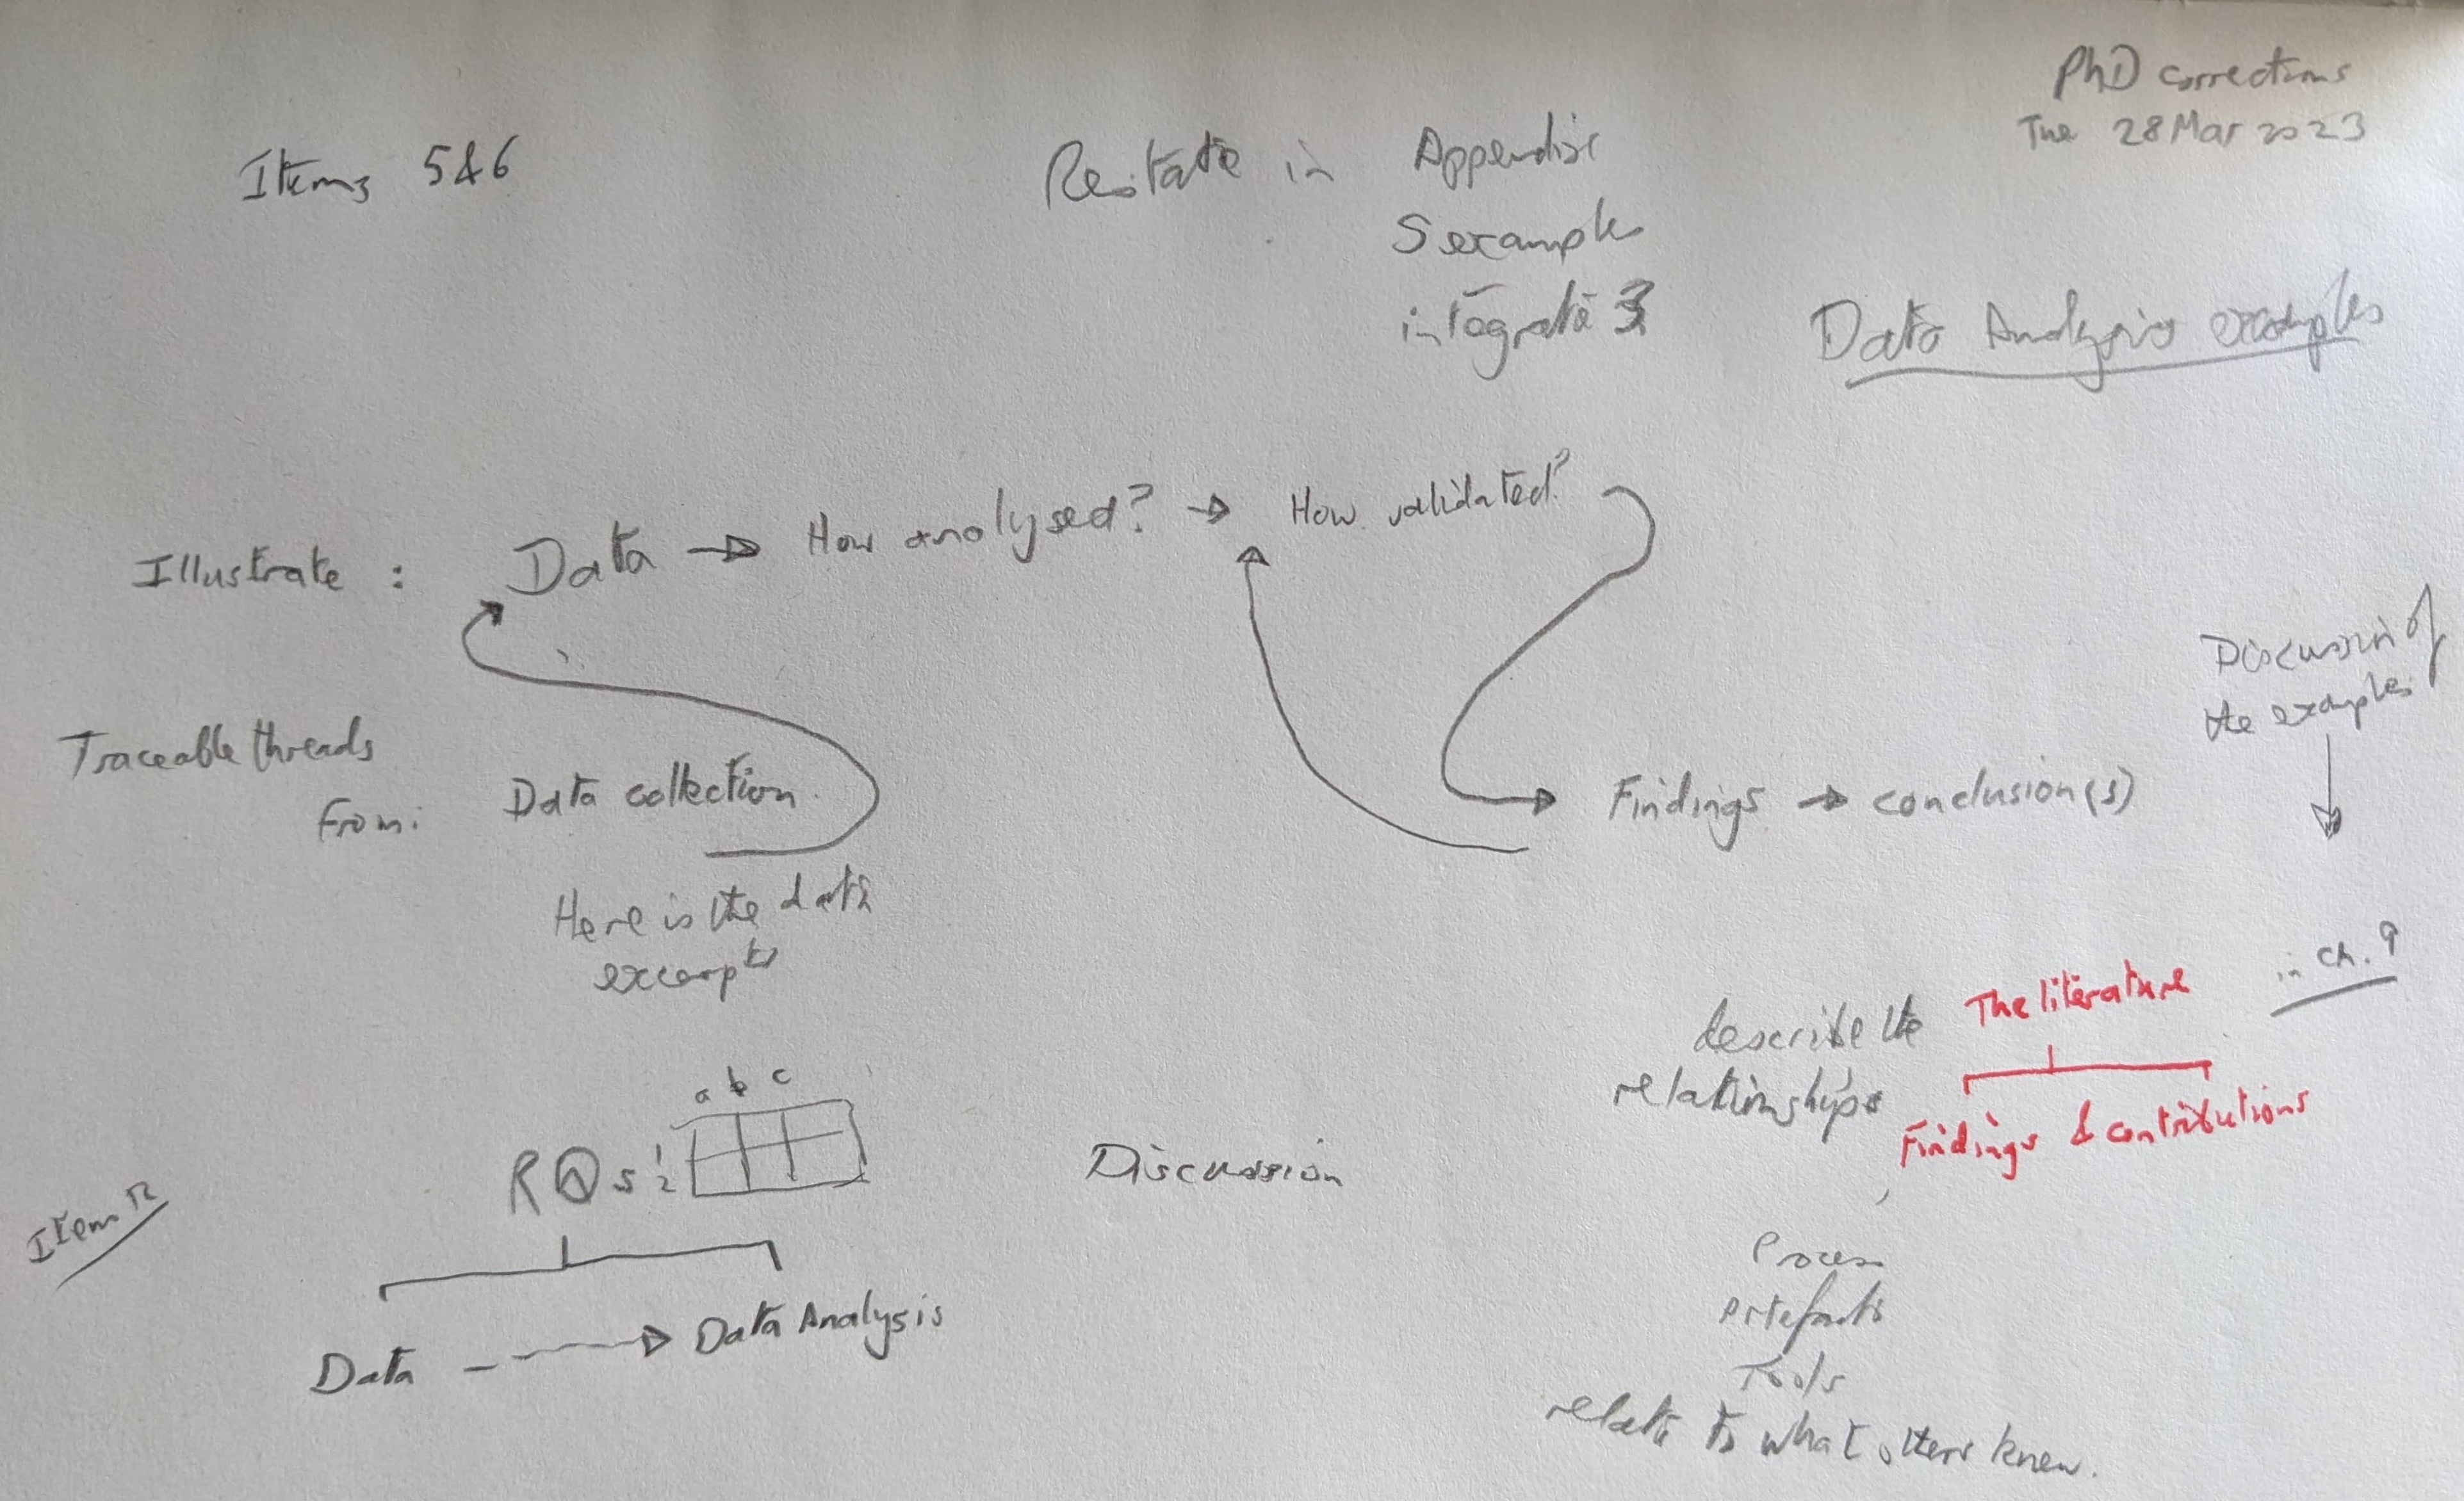
\includegraphics[width=\textwidth]{images/rough-sketches/worked-examples-in-context.jpg}
    \caption{Addressing - in part - items 5, 6, and 12}
    \label{fig:worked-examples-in-context}
\end{figure}

\section*{Context}
Items, 5, 6, and 12 in \secref{report-to-candidate-section} are repeated below, this appendix aims to address these items. Figure \ref{fig:worked-examples-in-context} illustrates my mapping of the connections and interactions that emerge from these items. Here a range of worked examples are provided for the interested reader, they reflect the approach and analysis of a multitude of findings that arose as part of this research. The mappings of findings are maintained using the spreadsheet design described in \secref{appendix-thematic-analysis}.

\begin{enumerate}
    \item[5] Clarify the data that was collected at each case study and how it was analysed and how it was validated, with illustrative data provided throughout.
    \item[6] More information is needed to clarify the research process i.e., to provide a clear link between the data collected, the findings and the conclusions drawn.
    \item[12] Provide more detail in the Appendices of the data and the data analysis done in relation to the RQs.
\end{enumerate}

\subsection*{Structure of each example}
The examples follow a consistent workflow which has been simplified to make the narrative clearer, the actual workflows for examples often included additional iterations, for example as more data was collected (some data arrived on an ongoing basis and bolstered with research-in-progress).

The structure is:

\begin{enumerate}

    \item Data, including how it was collected 
    \item Analysis, including how it was analysed
    \item Findings, and how they were validated
    \item Conclusions
\end{enumerate}

Candidate examples include:
\begin{itemize}
    \item \myindex{Kiwix} hackathon in Stockholm: where small changes led to an immediate and material improvement in reliability. 
    \item \myindex{Kiwix} experiment pre and post the hackathon: where comparisons in the experiment and the control apps indicate the improvements in reliability were achieved as a direct effect of making and releasing improved versions of apps.
    \item \myindex{PocketCode}\index{Catrobat} hackathon in Graz: this corroborates the pattern of results during and post hackathon. The results diverged from Kiwix after several months.\sidenote{Perhaps this could go before the Kiwix experiment, TBD}. In the discussion chapter incorporate the examples of how Moonpig actively managed reported crashes from Robospice, and from two homegrown bugs.
    \item Commercial project (\myindex{C1}): from release management reports through coding suitable tests, applying fixes, deploying the improved release. Also, third-party libraries (\myindex{OkHttp} in this example) deserve respect and attention to detail.\index{Third-party libraries!OkHttp}
    \item Three examples of scheduled automated emails from mobile analytics services (Sentry, Fabric Crashlytics, and whatever the one is that's eluding my memory right now). Also introduce Android Vitals automated emails and their infrequency. Cross referencing with Android Vitals reports. (via: \myindex{LocalHalo}, \myindex{Catrobat})
    \item Microsoft App Center's reports of future crashes. (via \myindex{C1}, \myindex{Micro experiments})
    \item Better bug reports by incorporating content from mobile analytics dashboards, including longevity of the contents of reports. (via \myindex{C1}, \myindex{Kiwix}, \myindex{GTAF}, and others).
    \item Coping with new Android releases using mobile analytics: \myindex{Moonpig}, \myindex{Third-party libraries!Robospice}, \myindex{SmartNavi}.
    \item \myindex{LocalHalo} \myindex{React Native!Expo framework} and the measurements performed by two mobile analytics services: \myindex{Sentry} and \myindex{Android Vitals} during the runtime problems.
\end{itemize}


\section[Kiwix experiment]{Kiwix experiment incorporating the hackathon in Stockholm}

\textbf{Data + how collected}: 
\begin{itemize}
    \item Android Vitals on-screen reports showing the failure (crash) rates.
    \item Source code pre- and post- changes to address crash clusters
    \item GitHub issue(s): \href{https://github.com/kiwix/kiwix-android/pull/1388}{The material contents of PR-1388, see lines 436 - 452.} TBD whether to include code snippets here:
    \item Contemporaneous conversations with app developers on the likelihood of being able to quickly and safely address the causes of two of the major sources of \glspl{glossary-crash-cluster}.
    \item Various notes
\end{itemize}
TODO add example screenshots, etc. here.



\begin{figure}
    \centering
    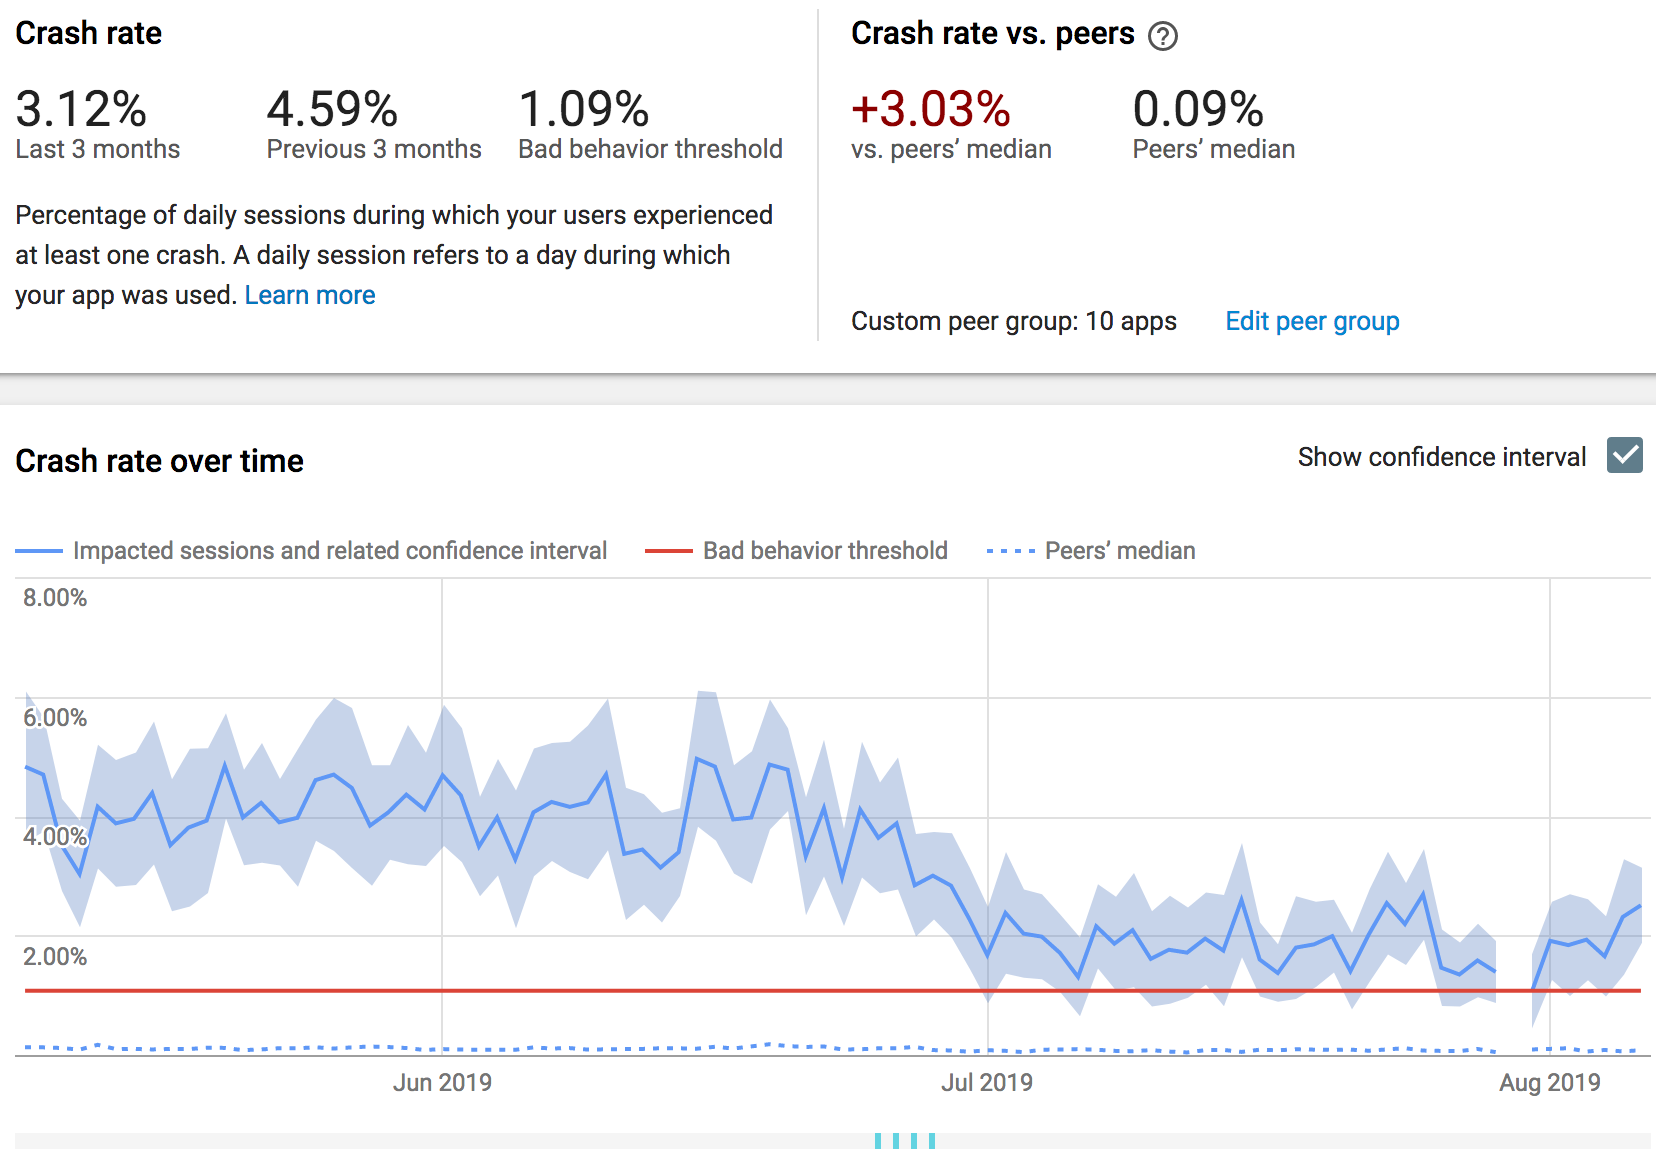
\includegraphics[width=\textwidth]{images/android-vitals-screenshots/kiwix/kiwix-crash-rate-drops-with-v2_5.png}
    \caption{Kiwix Crash rate drops with rollout of Version 2.5}
    \label{fig:kiwix-crash-rate-drops-with-v2_5}
\end{figure}

\textbf{Analysis + how it was analysed}: 
Straightforward investigation of the most prevalent failures, their probable contribution to the crash rate, the associated source code (identified from the corresponding stack traces).


\textbf{Findings, and how they were validated}: 
Ongoing reduction in crash rate as measured by Android Vitals. Validated through comparing crash rates for WikiMed and Kiwix over multiple releases of both apps.

The analysis was discussed with the technical lead of the Kiwix project and with three of the app developers. There was consensus throughout that the fixes were self-contained (with a low risk of adversely affecting any other aspect of the app's behaviour) and that the fixes were likely to be successful. Therefore it was agreed to perform the fixes and release the updated app that week.


\textbf{Conclusions}



\section[Kiwix experiment]{Kiwix experiment, pre- and post- Stockholm hackathon}

\textbf{Data + how collected}: included:
\begin{itemize}
    \item GitHub Issues, including:
    \begin{itemize}
        \item \href{https://github.com/kiwix/kiwix-android/issues/1426}{Proposal: to update the custom Android apps with bug-fixes on the 2.4 release}
        \item TBC
    \end{itemize}
    
\end{itemize}

\begin{figure}
    \centering
    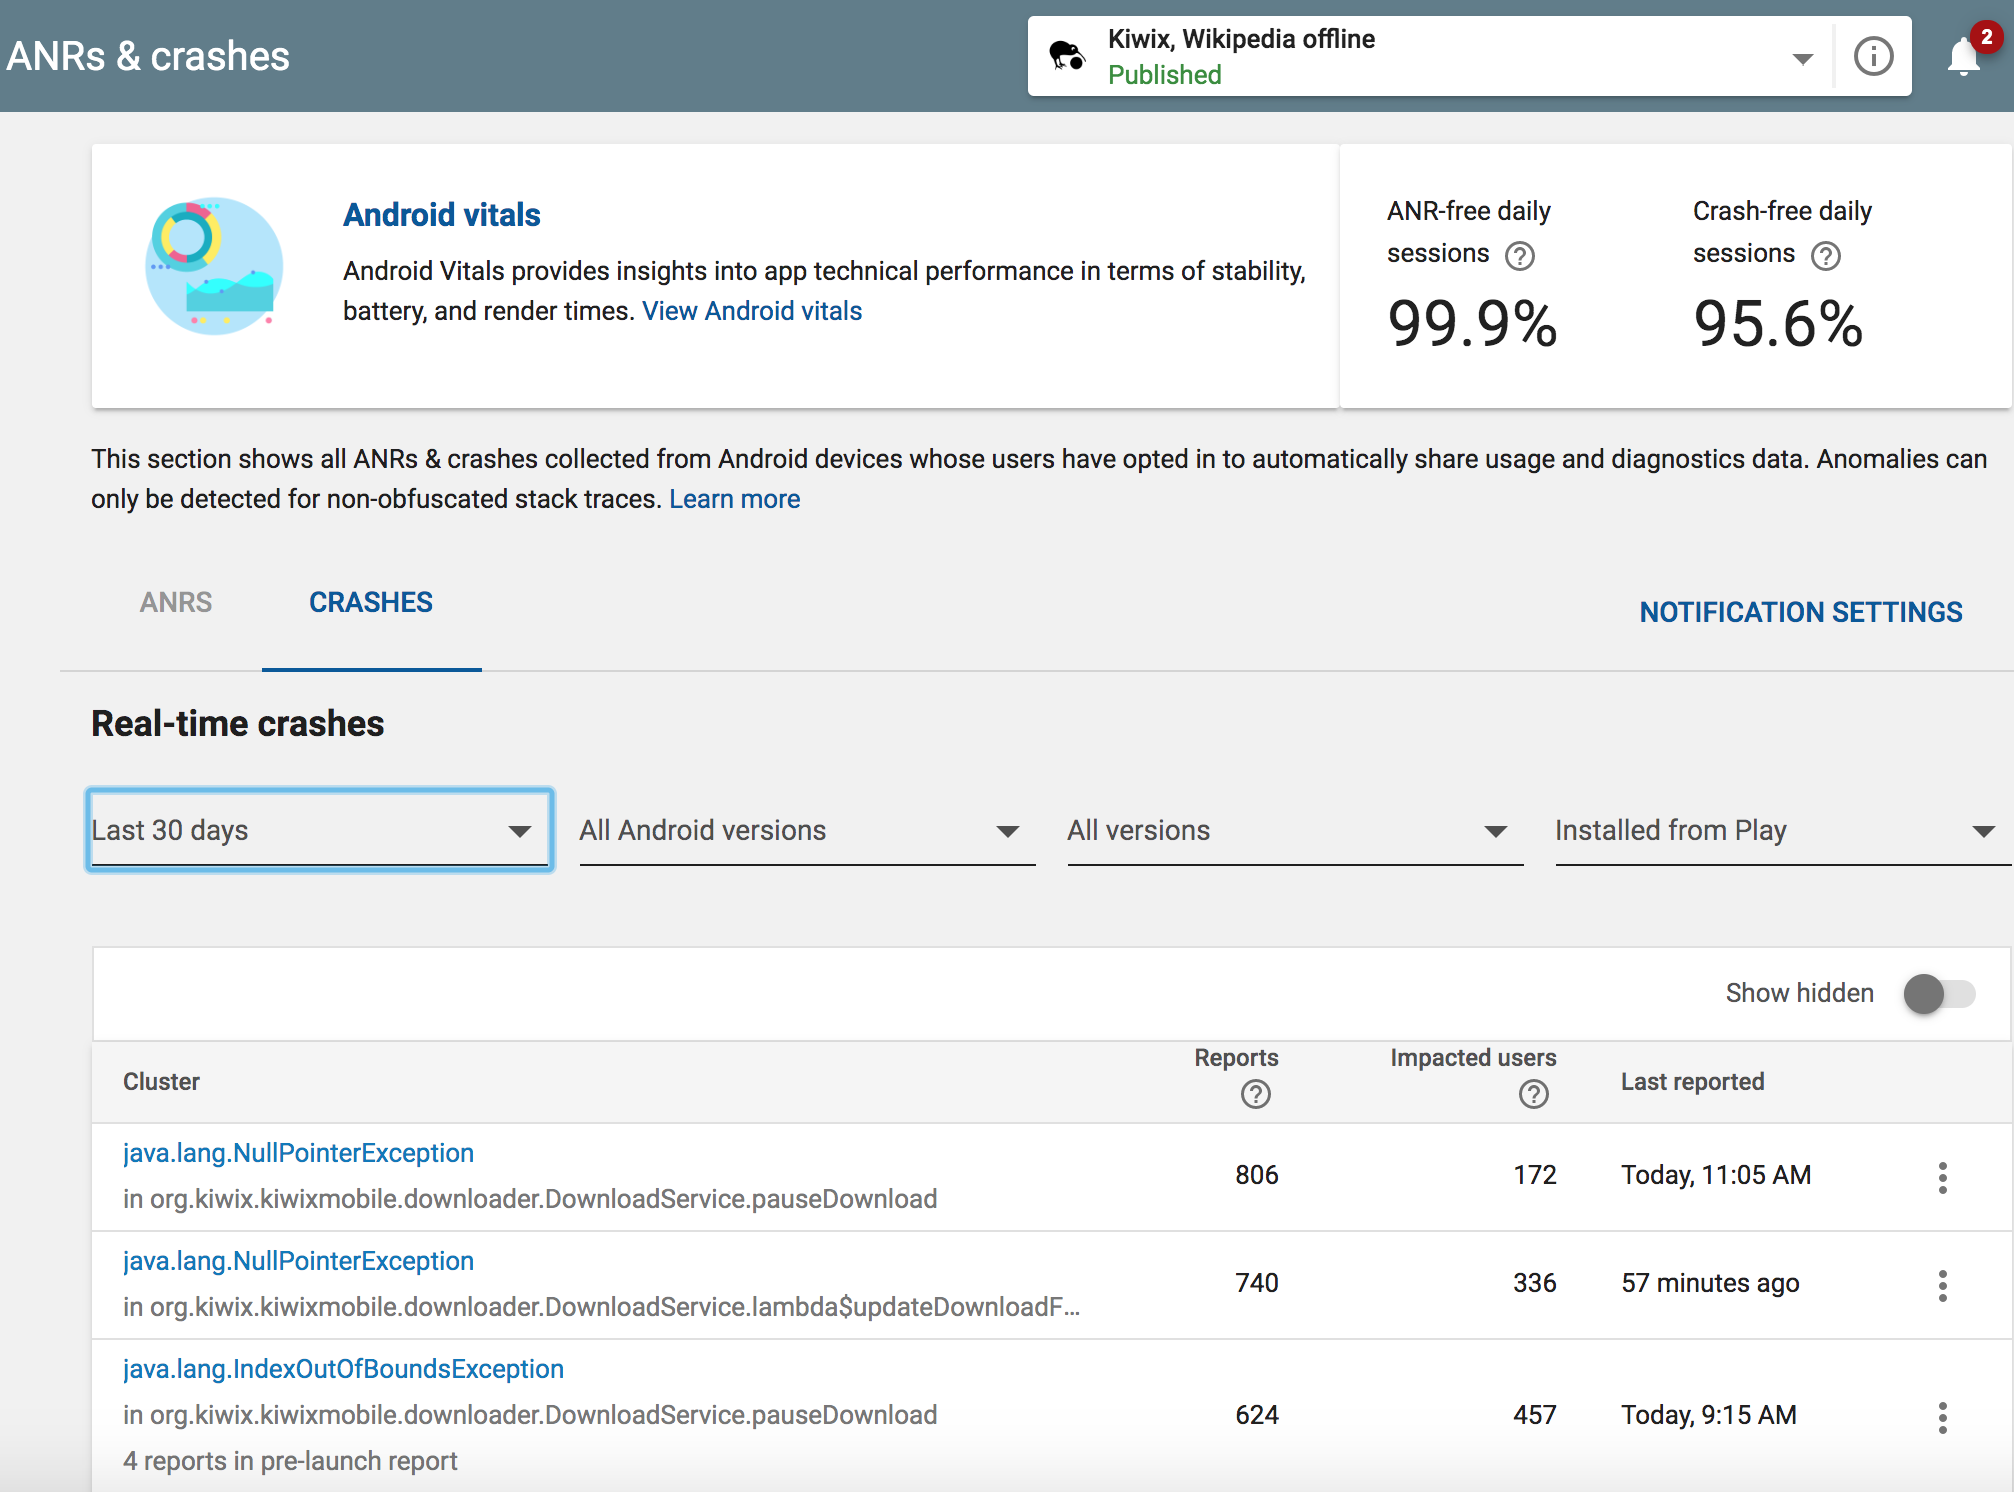
\includegraphics{images/android-vitals-screenshots/kiwix/Example-crash-clusters 10-jun-2019.png}
    \caption{Kiwix top crash clusters, recorded \nth{10} Jun 2019}
    \label{fig:example-kiwix-crash-clusters-10-jun-2019}
\end{figure}

\textbf{Analysis + how it was analysed}

\textbf{Findings, and how they were validated}

\textbf{Conclusions}


\section{Pocket Code Hackathon in Graz}

\textbf{Data + how collected}: 

\textbf{Analysis + how it was analysed}

\textbf{Findings, and how they were validated}

\textbf{Conclusions}


\section{Commercial project: OkHttp and Release Management}

\textbf{Data + how collected}: 

\textbf{Analysis + how it was analysed}

\textbf{Findings, and how they were validated}

\textbf{Conclusions}


\section{Automated emails from Mobile Analytics tools}

\textbf{Data + how collected}: 

\textbf{Analysis + how it was analysed}

\textbf{Findings, and how they were validated}

\textbf{Conclusions}


\section{Microsoft App Center and future dates}

\textbf{Data + how collected}: 

\textbf{Analysis + how it was analysed}

\textbf{Findings, and how they were validated}

\textbf{Conclusions}

Information was collected empirically.


\section{Better bug reports, longevity of reports}

\textbf{Data + how collected}: 

\textbf{Analysis + how it was analysed}

\textbf{Findings, and how they were validated}

\textbf{Conclusions}


\section{New Android, new issues, now what?}

\textbf{Data + how collected}: 

\textbf{Analysis + how it was analysed}

\textbf{Findings, and how they were validated}

\textbf{Conclusions}


\section{Crashes in cross-platform containers}

\textbf{Data + how collected}: 

\textbf{Analysis + how it was analysed}

\textbf{Findings, and how they were validated}

\textbf{Conclusions}

\section{Additional analysis examples}~\label{appendix-additional-analysis-section}

\begin{figure*}
    \centering
    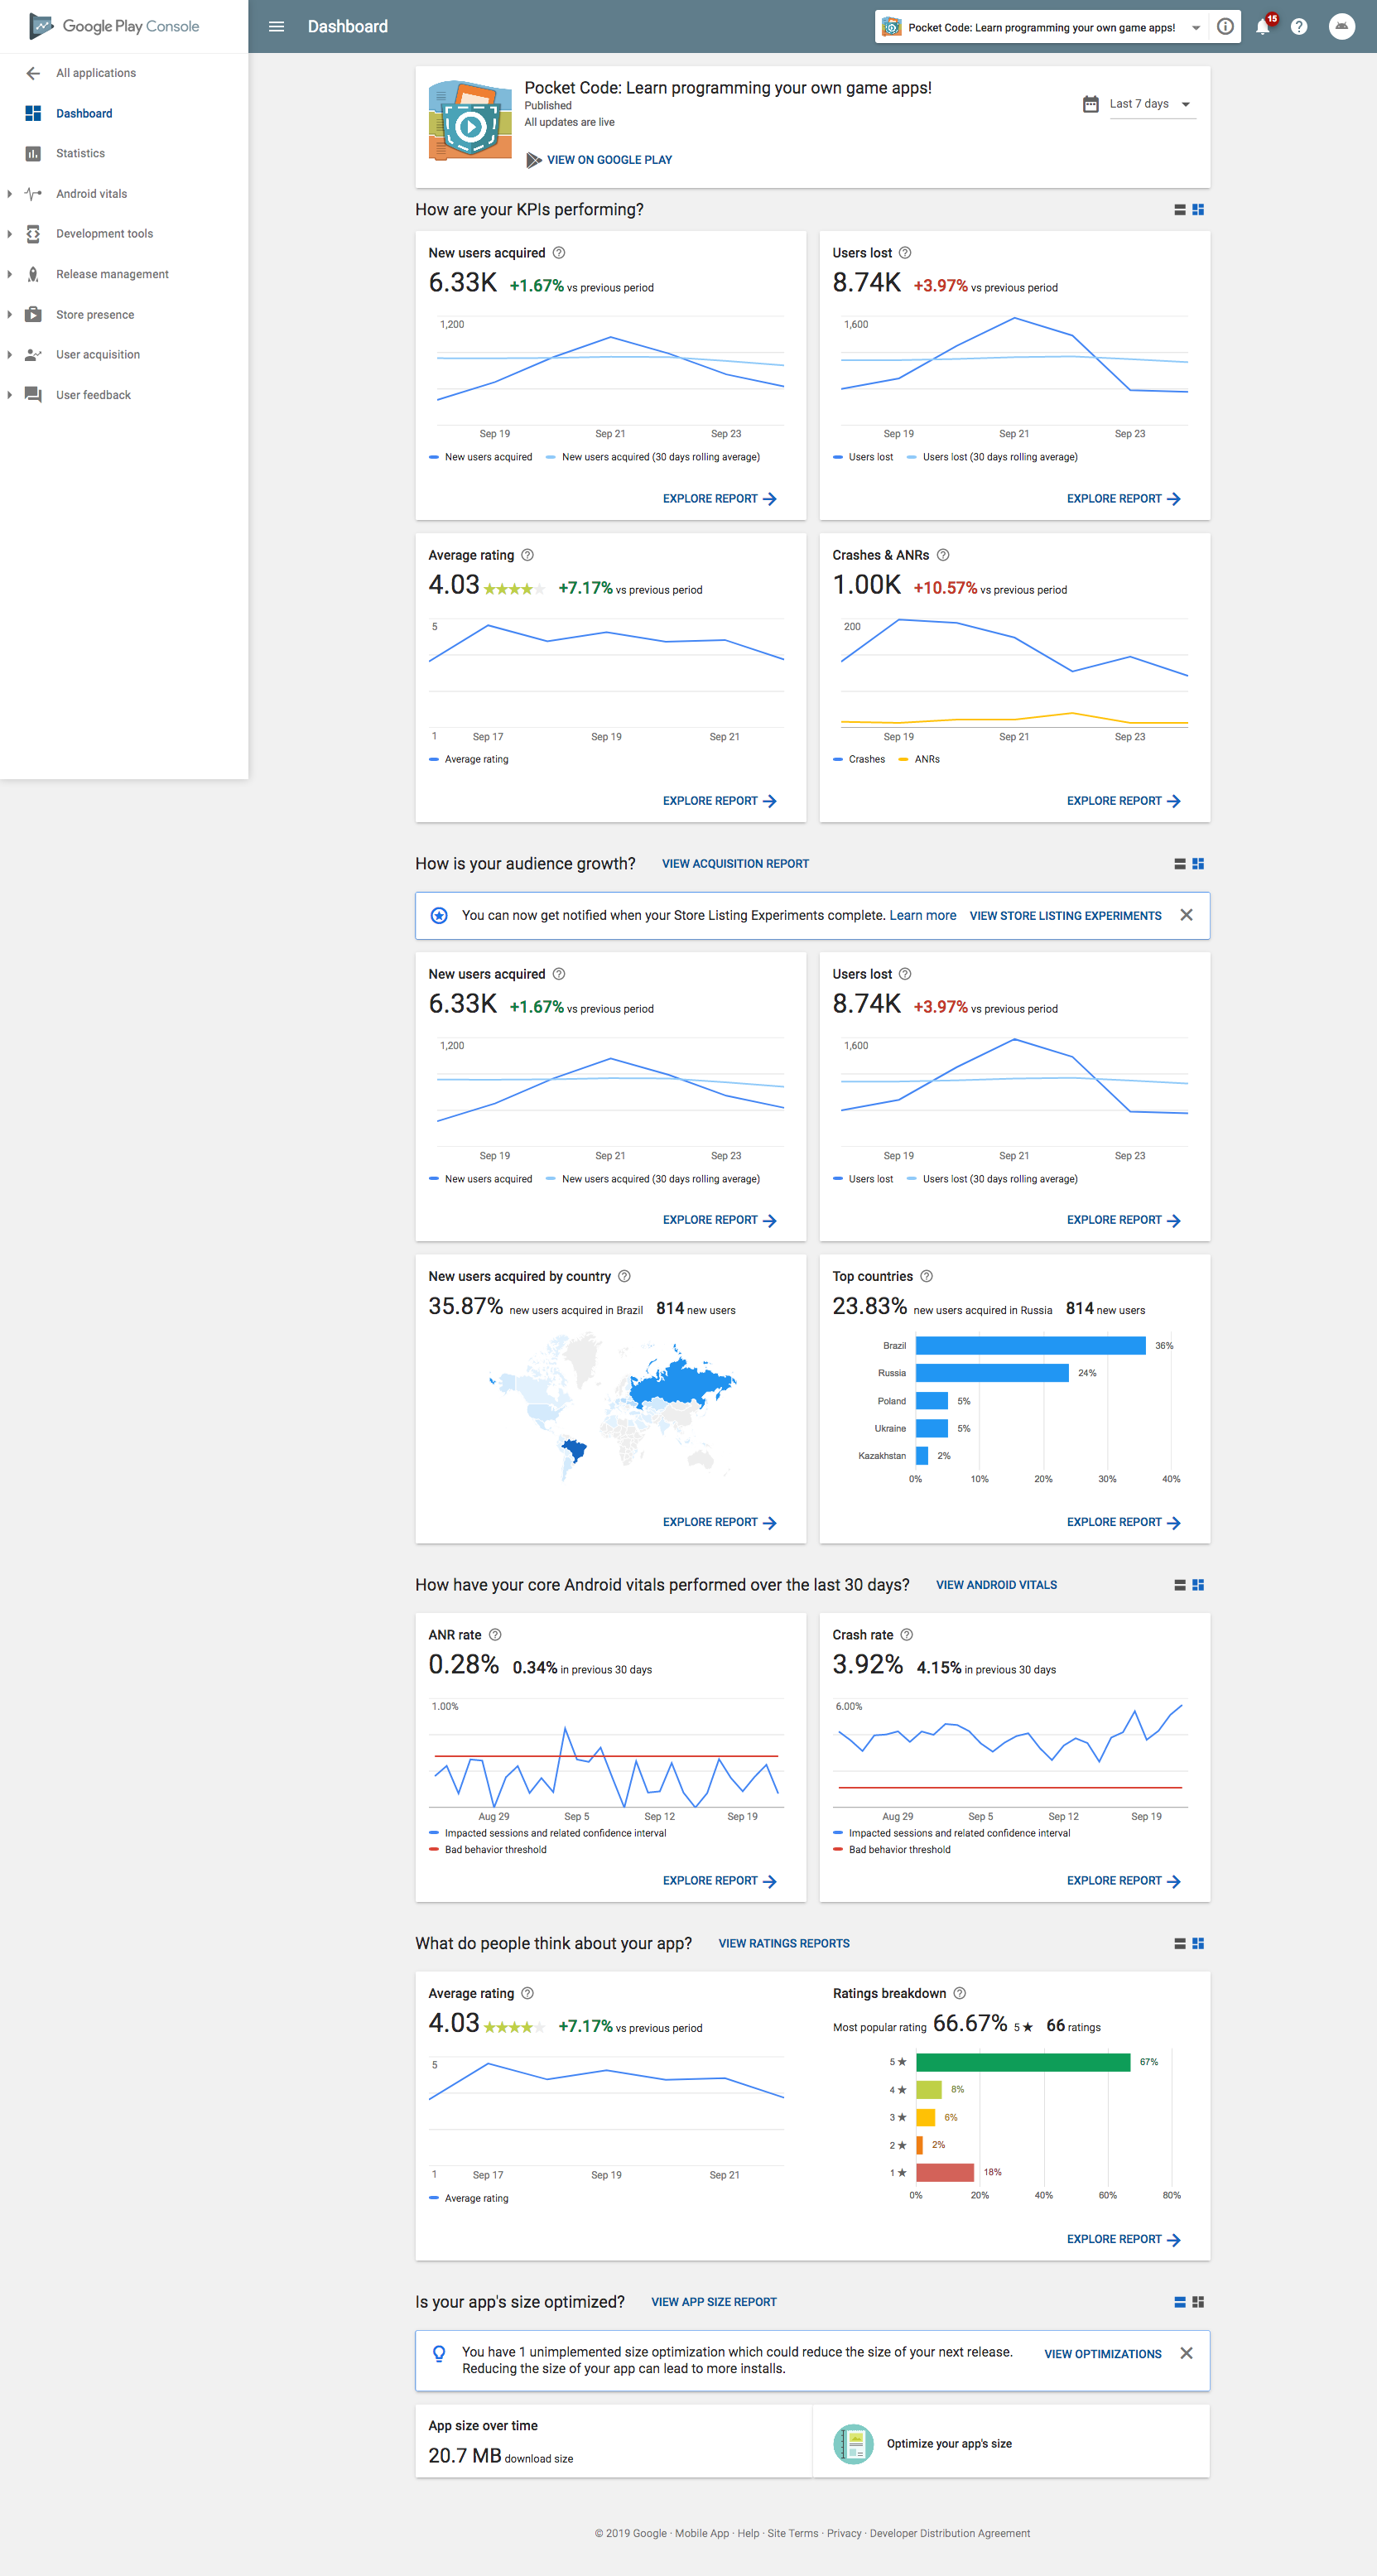
\includegraphics{images/android-vitals-screenshots/catrobat/1K crashes and ANRs in last 7 days Screenshot_2019-09-25 Dashboard - Pocket Code Learn programming your own game apps - Google Play Console.png}
    \caption[Google Play Console Dashboard for Catrobat]{1K crashes and ANRs in last 7 days Screenshot 2019-09-25 Dashboard - Pocket Code - Google Play Console}
    \label{fig:gpc-dashboard-catrobat-for-analysis}
\end{figure*}

\textbf{Data + how collected}: The data consists of an extended screenshot of the dashboard report that Google Play Console displayed for Catrobat's \myindex{PocketCode} Android app. It was collected using Firefox for Mac's `Save screenshot' right-click menu. This is a single instance of over 50 screenshot images collected during the research and presented here as a typical example of the analysis described in this section.

\textbf{Analysis + how it was analysed}: This seemingly basic dashboard contains lots of information, especially if compared with other recordings of the dashboard for: other date ranges, this app on other dates, other apps for this developer account, apps for other developer accounts, and so on. Various salient perspectives of the contents follow.

\textit{Structure and content}: 
In Figure \ref{fig:gpc-dashboard-catrobat-for-analysis} the dashboard has 5 expandable sections, expansion is indicated in blue at the right of each section. For example, the top-most section `How are your KPIs performing?' is expanded, as are the 3 middle sections, unlike the bottom-most section ``Is your app's size optimized'' which is not expanded. Every instance of this dashboard contained an even number of graph elements. The developer can toggle the expansion/contraction of each section. Here let's number the individual graphs with odd numbers on the left and even on the right, in ascending order from top to bottom, so the top left graph is 1 and the bottom right graph is 12.

\begin{enumerate}
    \item \textbf{New users acquired}: 6.33K +1.67\% vs previous period. The graph has a single vertical bar labeled (1,200) of the 4 in the graph, and 3 dates labeled (Sep 19, Sep 21, Sep 23). New users acquired are plotted in blue and New users acquired (30 days rolling average) are plotted in light blue.
    \item \textbf{Users lost}: 8.74K +3.97\% vs previous period. The graph has a single vertical bar labeled (1,600) of the 4 in the graph, and 3 dates labeled (Sep 19, Sep 21, Sep 23). Users lost are plotted in blue and Users lost (30 days rolling average) are plotted in light blue.
    \item \textbf{Average rating}: 4.03 +7.17\% vs previous period. The graph has a two vertical bars labeled (1, 5) of the 4 in the graph, and 3 dates labeled (Sep 17, Sep 19, Sep 21). The daily average rating is plotted in blue.
    \item \textbf{Crashes \& ANRs}: 1.00K +10.57\% vs previous period. The graph has a single vertical bar labeled (200) of the 4 in the graph, and 3 dates labeled (Sep 19, Sep 21, Sep 23). Crashes are plotted in blue and ANRs in yellow.

    \vspace{0.2cm}
    \hrule
    \vspace{0.3cm}
      
    \item \textbf{New users acquired}: 6.33K +1.67\% vs previous period. The graph has a single vertical bar labeled (1,200) of the 4 in the graph, and 3 dates labeled (Sep 19, Sep 21, Sep 23). New users acquired are plotted in dark blue and New users acquired (30 days rolling average) are plotted in light blue.
    \item \textbf{Users lost}: 8.74K +3.97\% vs previous period. The graph has a single vertical bar labeled (1,600) of the 4 in the graph, and 3 dates labeled (Sep 19, Sep 21, Sep 23). Users lost are plotted in dark blue and Users lost (30 days rolling average) are plotted in light blue.
    \item \textbf{New users acquired by country}: 35.87\% new users acquired in Brazil 814 new users. A flat map of the world has colour highlighting where Brazil is the deepest shade of blue on the map, followed by Russia.
    \item \textbf{Top countries}: 23.83\% new users acquired in Russia 814 new users. An ordered horizontal bar chart with 5 blue rows is shown in descending order of new users. These are labeled on the left with the name of the country and on the right with a percentage, here these values are: Brazil 36\%, Russia 24\%, Poland 5\%, Ukraine 5\%, Kazakhstan 2\%
    
    \vspace{0.2cm}
    \hrule
    \vspace{0.3cm}
    
    \item \textbf{ANR rate}: 0.28\% 0.34\% in previous 30 days. The graph has a single vertical bar labeled (1.00\%) of the 4 in the graph, and 4 dates labeled (Aug 29, Sep 5, Sep 12, Sep 19). The daily \gls{anr} rate, titled `impacted sessions and related confidence interval' is plotted in dark blue. A horizontal red line is also plotted on the graph for the `bad behavior threshold'.
    \item \textbf{Crash rate}: 3.92\% 4.15\% in previous 30 days. The graph has a single vertical bar labeled (6.00\%) of the 4 in the graph, and 4 dates labeled (Aug 29, Sep 5, Sep 12, Sep 19). The daily crash rate, titled `impacted sessions and related confidence interval' is plotted in dark blue. A horizontal red line is also plotted on the graph for the `bad behavior threshold'.

    \item \textbf{Average rating}: 4.03 +7.17\% vs previous period. The graph has a two vertical bars labeled (1, 5) of the 4 in the graph, and 3 dates labeled (Sep 17, Sep 19, Sep 21). The daily average rating is plotted in blue.
    \item \textbf{Ratings breakdown}: Most popular rating 66.67\% 5* 66 ratings. An ordered horizontal bar chart with 5 rows is shown in descending order of star rating. These are labeled on the left with the star rating and on the right with a percentage, each has a distinct colour. Here the values and colours are: 5* green 67\%, 4* light green 8\%, 3* orange 6\%, 2* lighter red 2\%, darker red 18\%
    
    \vspace{0.2cm}
    \hrule
    \vspace{0.3cm}
    
\end{enumerate}

Figure \ref{fig:gpc-dashboard-catrobat-for-analysis} also includes a header section that incorporates a calendar dropdown, showing Last 7 days here, and a link to the public page for the current app. In the `How is your audience growth?' grouping there is a link to `VIEW ACQUISITION REPORT' and a message regarding store listing experiments (a topic that's outside the scope of this research). The final unexpanded section `is your app's size optimized?' includes a link to `VIEW APP SIZE REPORT'. It also has a message about 1 unimplemented size optimization and a link to `VIEW OPTIMIZATIONS'; this is followed with the App size over time 20.7 MB download size.

\textit{Initial analysis}: In the interests of brevity some minor analysis has been excluded and some findings have been aggregated. 

\begin{itemize}
    \item \textbf{Dates}: the majority of the graphs are for the period selected in the header (last 7 days), however the two graphs for Android vitals are for 30 days, and the app size does not appear to have a period specified.
    \item \textbf{Duplicated graphs}: 3 graphs were duplicated in this dashboard: 1) new users acquired, users lost, and average rating. The duplication appears wasteful. The graphs often lacked information about the value represented by the lowest line on the vertical (Y) axis. The graph lines did display the value for each data point so the scale could be calculated, nonetheless the value of the baseline needs to be determined rather than being easily available.
    \item \textbf{Plausibility}: 8.74K users lost is more than the 6.33K new users acquired. If these figures refer to a userbase in common then the overall userbase has declined by 2.41K users in 7 days. No mention is made of returning users who were 'lost' who are now 'found' again, so there appears to be a possible gap in the overall picture of the userbase. Nonetheless, any app that loses more users than it gains would end up with close to no users at all.
    \item \textbf{Second-ranked country highlighted in top countries graph}: The top countries graph presents the results of the second-ranked country (Russia) rather than the first-ranked (Brazil), as per the graph immediately to the left/preceding this graph. 
    \item \textbf{Consistency}: 1) the date ranges are not consistent for all the graphs in the dashboard report. Android Vitals graphs have only been seen with a 30-day range\sidenote{Potentially some other users of Google Play Console are presented with other ranges so we cannot generalise beyond identifying that for every app and for every team and for every example the range has been 30-days for these graphs.}. 2) the counts for users are not consistent across the 4 graphs grouped under audience growth. Are there 6.33K new users or 814? or does 814 represent the new users in Brazil and/or in Russia?
    \item \textbf{Utility}: The Crashes \& ANRs graph presents both data sets on a common chart. [How] can these be usefully compared and contrasted? 
    \item \textbf{Freshness}: The Ratings graph is for a different date range (16 to 22 Sep 2019), two days earlier than the rest of the 7-day graphs (18 - 24 Sep 2019). 
\end{itemize}

\textbf{Findings, and how they were validated}
This and other similar dashboard reports for Kiwix and Catrobat, in particular, were analysed using the sense-making methods described in \ref{methodology-sense-making-method}\index{Sense-making}. Figure \ref{fig:wikimed-japan-top-countries} provides a succinct clear example which corroborates one of the findings where the second-ranked country - China - is the headline for the Japanese language version of the Wiki-Medicine app. 

Beacon-finding, described in \ref{section-beacon-finding-method}\index{Beacon-finding} identified dates and points on the various graphs. 

\begin{figure}
    \centering
    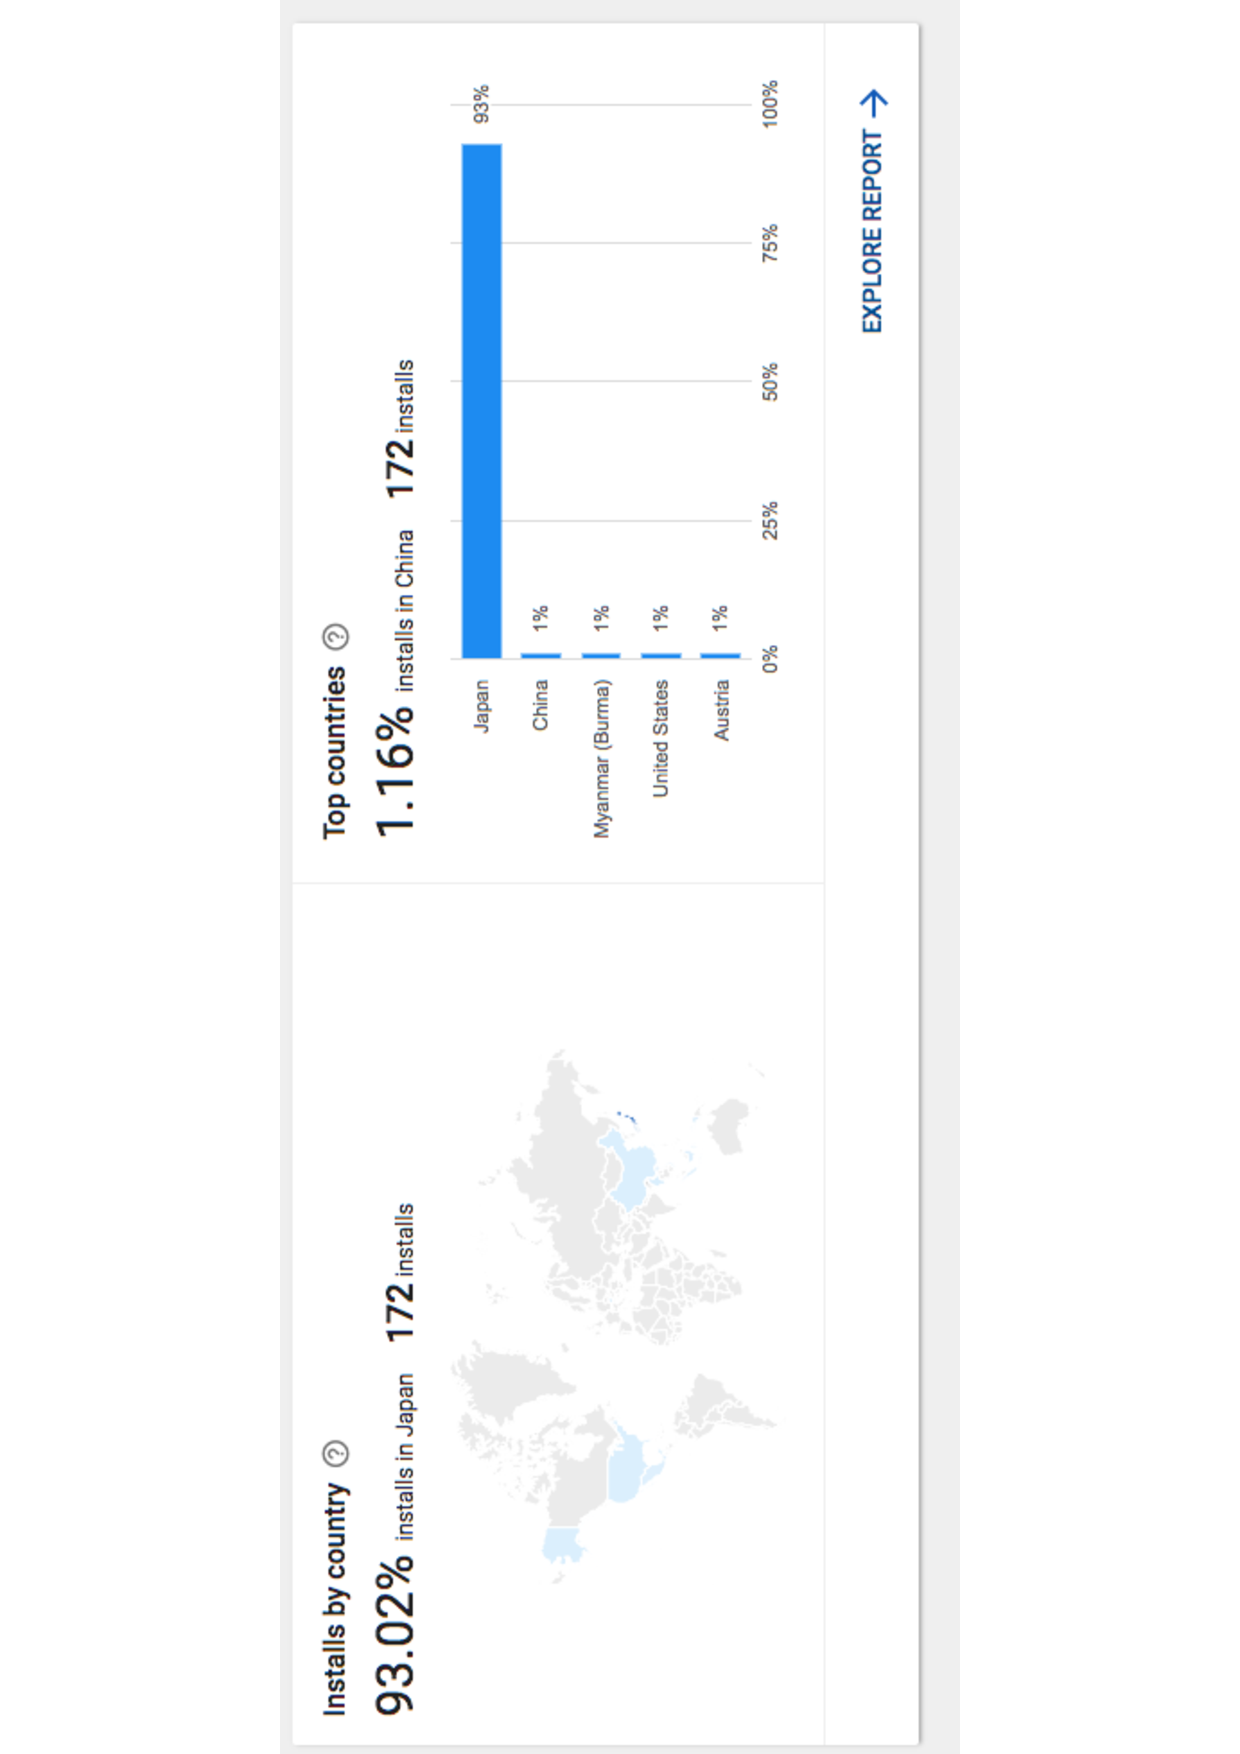
\includegraphics{images/android-vitals-screenshots/kiwix/wikimed-japan-top-countries.pdf}
    \caption{Kiwix: WikiMed in Japanese: Top Countries}
    \label{fig:wikimed-japan-top-countries}
\end{figure}

Drill-down into the graphs and reports linked from the respective graphs uncovered additional findings, including further differences in date ranges. The findings were presented to and jointly analysed with the Google Engineering team using the `ask the tool devs' method, described in \ref{section-ask-the-tool-devs-research-method}. They requested a report which I provided that categorised the findings. They validated the findings through discussions and email correspondence with Fergus Hurley the Product Manager of Google Play Console (who was acknowledged with his agreement in \sidecite{harty_google_play_console_insightful_development_using_android_vitals_and_pre_launch_reports}).

\textbf{Conclusions}